	The cameras are each synchronized to UTC time using the audio data and PCB log file.  Once each camera is synchronized to UTC time, frames are extracted at regular intervals for each video, and these images are said to be ``synchronized.''  These videos are not however, hardware triggered and therefore the shutters are not synchronized.  The theoretical accuracy of this methodology results in the cameras synchronized to a worst case scenario of 1/30s when ignoring all other sources of noise.
	
	\section{Technical Approach}
	The algorithm to develop the synchronization of the cameras from GoPro time to UTC time was developped in Matlab.  The logfile, as described in Section \ref{sec:algoLog}, records the GPS data, PPS rising edge time, and the time the binary count value was sent to the GoPro.  The GoPro audio channels recorded the PPS signal and the binary count value from the Teensy microcontroller.  Each of these data has redundant observations between the time frames, which enable us to perform a least squares adjustment between each of the time frames.  When the processing is complete, p1 and p2 coefficient values as described in \eqnref{eqn:utc2gopro}, are recorded in a text file.
	
	\begin{equation}
	\label{eqn:utc2gopro}
	t_{UTC} = p1 \times t_{gopro} + p2 
	\end{equation}
	
	The processing is broken up into four main algorithms:
	\begin{enumerate}
		\item Calculate GoPro time to UTC time coefficients
		\item Extract Frames from GoPro Video at UTC times 
		\item Convert logfile into a CSV file with GPS info and UTC timestamps
		\item Interpolate GPS position info for each image based on corresponding UTC times 
	\end{enumerate}

	\subsection{GoPro to UTC time}
	
	\subsubsection{GoPro Audio Signal Decoding}

	One challenge with extracting the binary and PPS data from the audio channel of the GoPro was filtering out the GoPro signal conditioning of the input signal.  For example, \figref{fig:rawPPS} demonstrates how a square PPS signal appears in the recorded audio file.  Notice how the PPS signal, which should be a square wave, actually decays to 0 despite the voltage.  Therefore, an algorithm was written to detect large changes in signal, which then represent changes in voltage.  For the PPS signal, the detection of rising and falling edges of the PPS pulse was trivial, but it became slightly more complicated for the binary signal.
	\begin{figure}[H]
		\centering
		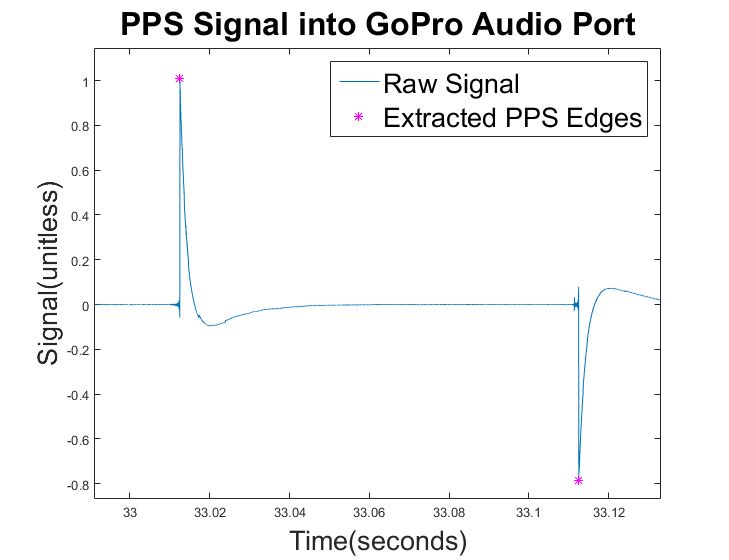
\includegraphics[scale = 0.7]{../figures/rawPPS.png}
		\caption{The PPS, which should be represented as a square wave, actually decays to 0 regardless of the voltage. The algorithm therefore is written to detect the large gradients, which represent a change in voltage.}
		\label{fig:rawPPS}
	\end{figure}
	The binary signal is set to 300 baud in the Teensy algorithm however it actually is sent at 1660 baud.  This is acceptable, as the peaks were still discernable at this baud rate.  If however, a faster baud rate were used, the peaks would become too close together and be difficult to decode.  \figref{fig:rawNMEA} is an example decoded binary signal.  The data is sent at 8N1 with no parity, so for the 2 byte binary integer being sent, it uses 20 bits.  The raw signal is filtered to detect large changes, then a Gaussian filter is applied to smooth out the data.  The peaks are then extracted at the known baud rate, with a peak threshold set as 1/3 the absolute value of the max peak value.  The signal is then decoded into a binary signal, using an algorithm that takes into account that the signal will only change when the bit is changing.  For example, notice how the 17th bit is high, and the 18th bit is 0, but both those values represent a 1 in binary.  The bit value does not change to 0 until a low peak is detected at bit 19.  
	
	\begin{figure}[H]
		\centering
		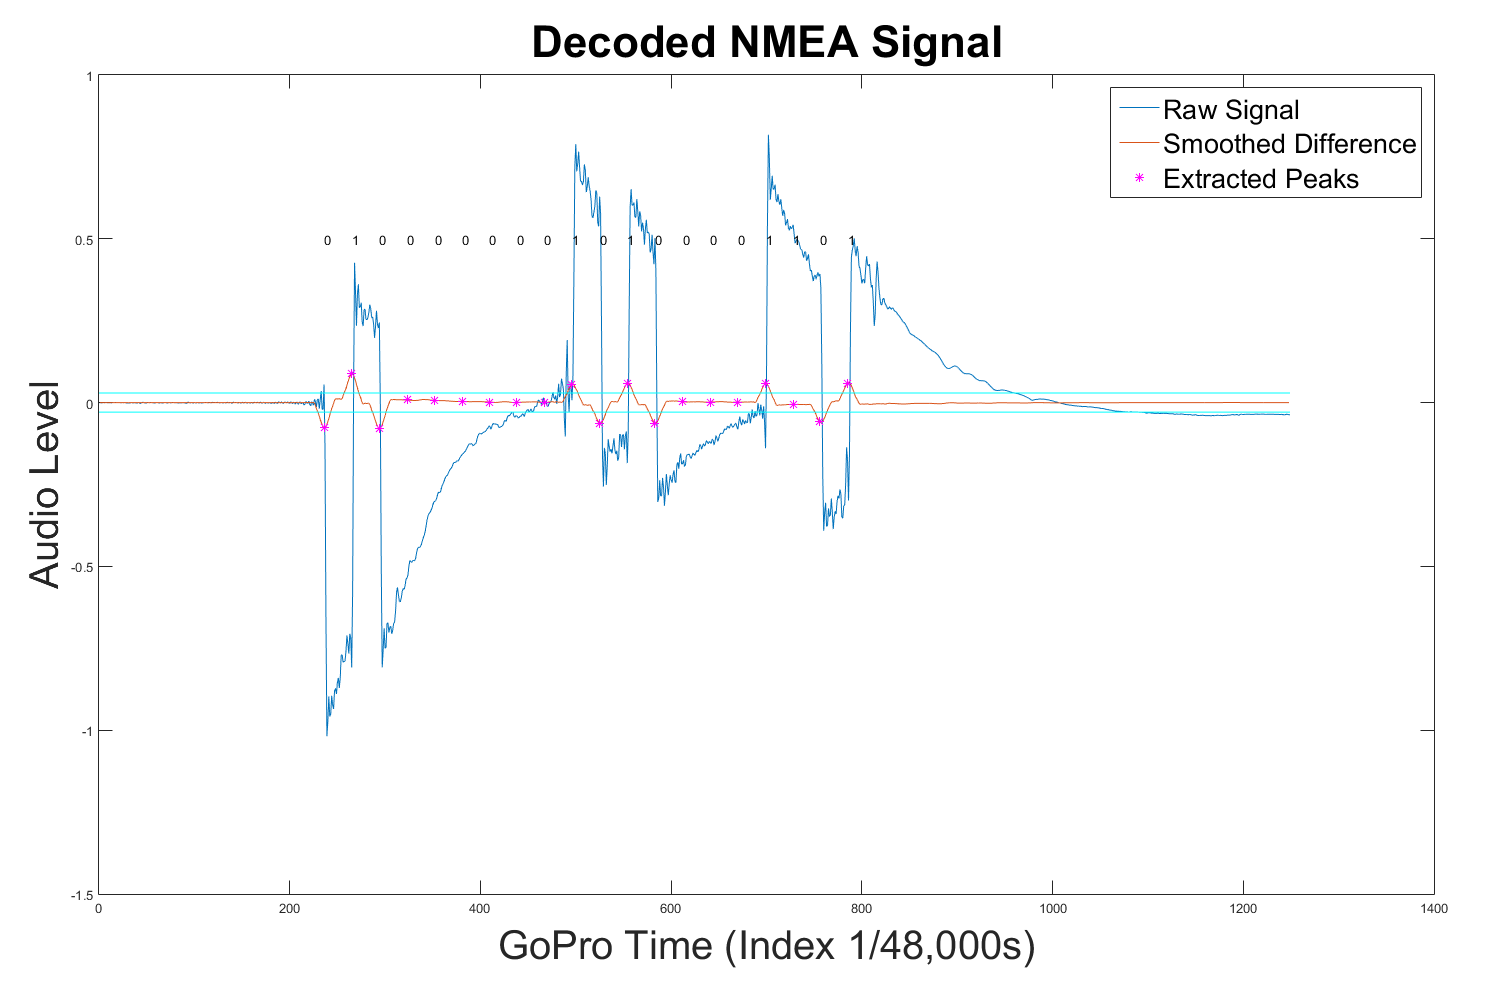
\includegraphics[scale = 0.4]{../figures/decodedNMEA.png}
		\caption{The binary signal sent to the audio port suffers the same decay as shown in the PPS signal.  Here, the change in signal was used to detect when a change in bit value occurred.}
		\label{fig:rawNMEA}
	\end{figure}
	
	\subsubsection{Algorithm Pseudocode}
		The conversion from GoPro time to UTC time can be performed without a PPS signal, but the absolute quality of this conversion will suffer due to latency in the Serial NMEA port and buffering.  However, the relative synchronization between the cameras should remain the same, as any latency in reading the Serial port will be constant across each camera.  The different time frames and data exchange between the Teensy, GoPro, and GPS PPS are shown in \tabref{tab:timeframes}.  Note that there is an ambiguity when attempting to correlate two PPS signals, as the PPS signal simply refers to a start of a second.  If two PPS triggers are detected in two different time frames, there is no direct way to correlate the two.  For this reason, GPS data sends NMEA strings to put the PPS second into an absolute UTC time frame.  The function to calculate this offset and save a text file has been electronically delivered, and is also shown in \ref{sec:calcGopro2GPStime}.  
	
		\begin{table}[htbp]
			\centering
			\caption{The different data exchanges are recorded in three different time frames.  Note that the X represents a direct correspondence between the data, while a `*' represents an ambiguity in the correspondence. The PPS values are sent at the beginning of each second in time, but there is no context to what actual second it is.}
			\begin{tabular}{| l | c | c | c |}
				\hline
				Time Frame & Index & GPS NMEA & GPS PPS \\
				\hline
				GoPro & X     &       & * \\ 			\hline
				Teensy & X     & X     & X \\ 			\hline 
				UTC   &       & X     & * \\
				\hline
			\end{tabular}%
			\label{tab:timeframes}%
		\end{table}%
		
		The steps to achieve time synchronization between GoPro time and UTC time are outlined below:
		\begin{enumerate}
		\item Extract All data from the SD card and the GoPro Audio
		\item Use correspondences between Teensy Time and GoPro time for the index counter sent to the audio channel to calculate the conversion between the two time frames.
		\item Use the NMEA GPS string recorded in Teensy time and stamped with UTC time to calculate a conversion between Teensy time and UTC time.  *NOTE, if no PPS is detected, the algorithm stops here
		\item A PPS pulse is described as having a rising edge exactly on the second with precision to the nanosecond.  Using this knowledge, and the PPS timestamps in Teensy Time, estimate each PPS time in UTC time.  Round the value to the nearest second after using the Teensy to UTC conversion
		\item Convert the GoPro PPS times to UTC time, and round to the nearest PPS in UTC time.  This assumes that the time is accurate to less than 0.5 seconds, so that the rounding does not become out of phase.
		\item Calculate a new conversion from GoPro time to UTC time using the PPS correspondences.
		\item Save this information to a text file `*\_gopro2gps.txt.'
		\end{enumerate}
	
	\subsection{Extract Frames}
	Frames are extracted from the video imagery using the known conversion from GoPro time to UTC time, and a user-defined vector containing the times to extract imagery at.  The algorithm to extract these frames and save imagery and metadata is provided electronically and also located in \ref{sec:extractFrames}. The pseudocode for the algorithm to extract frames is as follows:
	\begin{enumerate}
		\item Read the MP4 Video file into Matlab using Matlab's \textit{VideoReader} Class
		\item Read the previously calculated goPro to UTC time constants
		\item Using the user input vector of desired UTC times for frames, calculate the correct frame indices to extract imagery
		\item Write each frame to a JPG in a user defined folder, and save an `iminfo.txt' CSV file which contains 3 Columns.  In order to quantify the timing errors, the actual and desired times are both written.  An example output file is shown in \figref{fig:iminfo}
		\begin{itemize}
			\item Image Name
			\item Image Actual Time (This is the actual time of the frame)
			\item Image Desired Time (This is the time the user wanted the frame at)
		\end{itemize}
	\end{enumerate} 
	
	\begin{figure}[H]
		\centering
		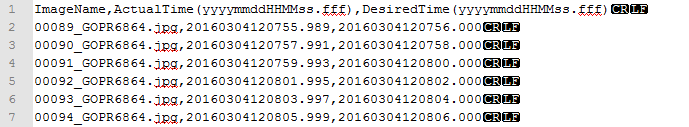
\includegraphics[scale = 0.8]{../figures/iminfotxt.png}
		\caption{The image info text file is comma delimited and is used to store metadata about the extract video frames.}
		\label{fig:iminfo}
	\end{figure}
	
	One issue that arose is that Windows machines running operating systems that predate Windows 10 do not contain the codecs for reading 4K video by default.  Since Matlab relies on these codecs, the Matlab \textit{VideoReader} class throws an error when attempting to read a 4K video file.  This issue is alleviated by instaling 3rd party codecs.
	
	A second issue that may arise is the use of the \textit{read} function is flagged bt Matlab as subject to removal in future versions of Matlab.  This function is used, rather than the new \textit{readFrame} function, as the \textit{read} function enables a frame to be read based on an index value.  The \textit{readFrame} function requires you to read each frame sequentially, which takes a lot of unnecessary time when you are reading every N frames.  
	\subsection{Convert Log file to CSV}
	\label{ssec:convertLog2CSV}
	The log file that is recorded on the SD card contains L1 GPS data which can be used to provide an initialization for the camera position when running Structure from Motion algorithms.  A quick algorithm to decode the log file and convert it from NMEA to a more easily interpretted CSV is provided electronically.  An example resultant file is shown in \figref{fig:gpstxt}.  This file is simply raw time and GPS position data, but it can be leveraged to interpolate camera positions, as described in \ref{ssec:InterpGPS}.
	
	\begin{figure}[H]
		\centering
		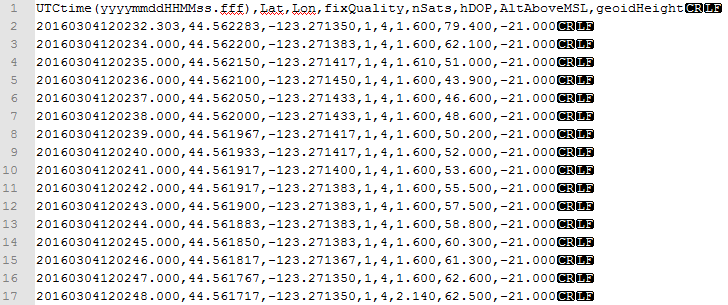
\includegraphics[scale = 0.6]{../figures/gpstxt.png}
		\caption{The log file is turned into a CSV file so that the GPS data can be easily extracted and leveraged.}
		\label{fig:gpstxt}
	\end{figure}
	
	\subsection{Interpolate GPS data for each image}
	\label{ssec:InterpGPS}
	Once all of the imagery has been extracted, estimated camera pose positions can be calculated using various sources of GPS data.  \figref{fig:postxt} demonstrates an example metadata file generated from the logfile gps positions.  The algorithm, shown in \ref{sec:addPositionInfo}, is developped to be modular so that any CSV file can be used to add position or other temporal metadata to the imagery.  The CSV file must have:
	\begin{enumerate}[a)]
		\item headers to describe the data, as these are propagated through to the merged metadata file
		\item A first column representing UTC time in the format `yyyymmddHHMMss.fff.'
	\end{enumerate}
	If these parameters are met, other sensor data such as that from the autopilot can be easily integrated into the workflow.
	
	\begin{figure}[H]
		\centering
		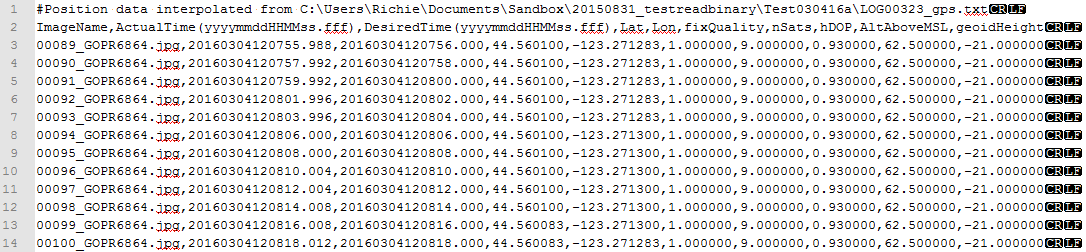
\includegraphics[scale = 0.6]{../figures/postxt.png}
		\caption{The GPS data is appended to the image position metadata so that each image has interpolated GPS values.}
		\label{fig:postxt}
	\end{figure}
	
	\section{Temporal Accuracy}
	The temporal accuracy was tested by observing a cell phone that was updating with the UTC time via a website.  This test is limited greatly by a number of factors, included refresh rate of the phone screen, refresh rate of the website, and the displayed temporal resolution of the website is only to the second.  Initial results show that the time is correctly synchronized to UTC time, in the sense that the times appear to match relatively well with what is shown on the screen, as shown in \figref{fig:badsync}.
	
	\begin{figure}[H]
		\centering
		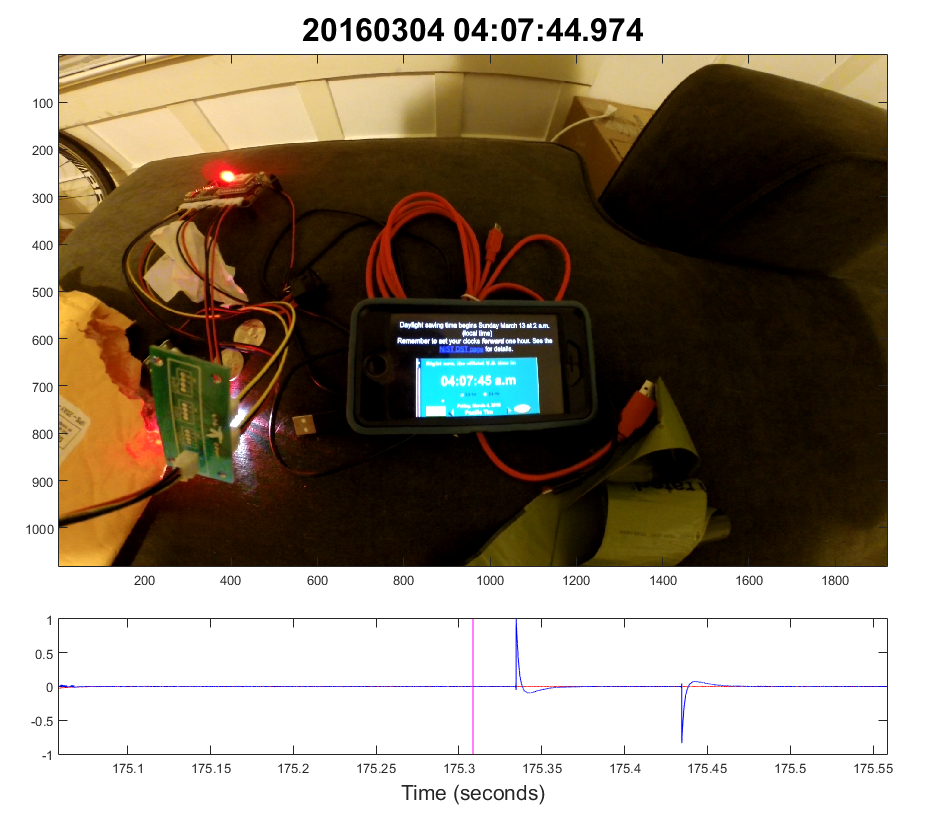
\includegraphics[scale = 0.6]{../figures/badsync.png}
		\caption{The synchronization of the imagery was tested using a cell phone updating via a time server to UTC time.  The top pannel shows the imagery, and the bottom panel shows the PPS signal channel of the audio.  The magenta line represents the current time. Notice that the white, PPS light under the green PCB is on, before the signal is shown in the audio.}
		\label{fig:badsync}
	\end{figure}
	
	However, one issue that was observed is the latency between the video and the audio channel within the GoPro.  GoPro cameras are consumer grade cameras, and therefore time synchronization between the audio and video does not need to be perfectly precise.  Notice in \figref{fig:badsync} how the white PPS light under the PCB is lit up before it is recorded on the audio channel.  This indicates that the Video signal is farther ahead in time than the audio channel.  This offset was observed to be consistently one to two frames off, but further tests would need to be done to make any statements about it's consistency.  Hopefully, the latency between the audio and video port is a constant offset that can be calculated once and applied to each camera.  Further tests will need to be done to fully quantify the accuracy of this methodology due to other sources of error.	
	
	\section{Possible Improvements}
	\subsection{Embed x8 Flight log info}
	The X8 Pixhawk autopilot records position and orientation values directly to the SD card in the Pixhawk.  These data can be read into the 3D Robotics ``Mission Planner'' software, and converted into a Matlab file.  Once the data is in Matlab, it should be saved as a CSV, as described in \ref{ssec:convertLog2CSV}.  While the autopilot is not rigidly mounted to the cameras, it should provide a more accurate camera pose estimation than what could be derived from the onboard 9dof IMU.
	\subsection{Incorporate onboard IMU}
	If however, the vibration damping between the camera and the X8 autopilot significantly invalidates the ``rigid body'' assumption, the onboard IMU could be used to generate improved position and orientation values.  A Kalman filter should be implemented to generate an improved trajectory than what could be generated from just the raw data.  One issue that will need to be overcome in order to integrate this system, is to modify the Teensy code to record the raw 9dof measurements.  These raw values have been excluded from this iteration, as there was concern that reading and writing from another sensor could cause latency and delays in the time synchronization section of the code.  Further tests will be required to ensure that this is not the case.